\chapter{Системийн зохиомж}

\section{Архитектурын ерөнхий үндэслэл}

Энэхүү судалгааны ажлын хүрээнд хөгжүүлж буй annotation-д суурилсан dependency injection framework нь энгийн хэрэглээний программ бус, харин бусад программын ажиллагааг дэмжих суурь программ хангамжийн орчин буюу framework шинжтэй систем юм. Иймээс түүний архитектур нь зөвхөн модуль хуваарилалт төдий бус, харин объект илрүүлэлт, мета өгөгдөл уншилт, bean бүртгэл, объект үүсгэлт, хамаарал шийдэлт, алдаа боловсруулалт зэрэг дотоод механизмыг ойлгомжтой, өргөтгөх боломжтой, туршихад хялбар байдлаар зохион байгуулах шаардлагатай.

\section{Сонгосон архитектур: Давхаргат архитектур}

Энэхүү framework-ийн хэрэгжилтэд хамгийн тохиромжтой шийдэл нь давхаргат архитектур (Layered Architecture) гэж үзсэн. Учир нь уг судалгааны ажлын гол зорилго нь enterprise хэмжээний тархмал систем байгуулах бус, харин annotation болон reflection-д тулгуурласан IoC/DI механизмын дотоод ажиллагааг загварчлан хэрэгжүүлэхэд оршино.

Давхаргат архитектур нь системийн бүрэлдэхүүн хэсгүүдийн үүргийг тодорхой зааглаж, давхаргууд хоорондын хамаарлыг хязгаарласнаар өөрчлөлтийн нөлөөг багасгах, кодын уншигдах байдлыг сайжруулах, мөн тест хийх боломжийг нэмэгдүүлэх давуу талтай.\footnote{Microsoft, ``Layered (N-tier) Architecture'', \url{https://learn.microsoft.com/en-us/azure/architecture/guide/architecture-styles/n-tier}} 

\clearpage
\section{Сонгосон архитектурын давуу тал}

Энэхүү framework-д layered architecture ашигласнаар
дараах давуу талууд бий болно.

\begin{enumerate}
    \item \textbf{Annotation тодорхойлолт болон runtime логикийн
    тусгаарлалт.}
    \texttt{@Component}, \texttt{@Autowired} зэрэг annotation-ууд
    нь зөвхөн мета мэдээлэл агуулж, тэдгээрийг боловсруулах логик
    нь container болон injector давхаргад төвлөрнө.
    Ингэснээр annotation-ийн тодорхойлолтыг өөрчлөхгүйгээр
    боловсруулах логикийг бие даан өргөтгөх боломж бүрдэнэ.

    \item \textbf{Scanner давхаргын өргөтгөх чадвар.}
    Package scanning нь тусдаа давхарга болж байрласнаар
    \texttt{ClassPathScanner}-ийг цаашид JAR файл дэмжих,
    тусгай шүүлтүүр (\textit{filter}) нэмэх зэрэг
    хувилбаруудаар өргөтгөх боломж бүрдэнэ.

    \item \textbf{Мета өгөгдөл болон instance хадгалалтын
    тусгаарлалт.}
    \texttt{BeanDefinition} болон \texttt{BeanRegistry} нь
    тусдаа байснаар bean-ийн мета өгөгдөл болон
    runtime-д үүсгэгдсэн instance хадгалалтыг
    оновчтой зохион байгуулах, ирээдүйд бие даан
    сайжруулах боломж бүрдэнэ.

    \item \textbf{Fail-fast зарчмын хэрэгжилт.}
    Exception давхаргыг тусгаарласнаар систем нь алдааг
    аль болох эрт, тодорхой мэдэгдлийн хамт илрүүлдэг
    \textit{fail-fast} шинж чанартай болно.
    Энэ нь хөгжүүлэгчид алдааны шалтгааныг хурдан
    ойлгоход тустай.

    \item \textbf{Spring Framework-ийн архитектурын суурь
    ойлголттой нийцэл.}
    Энэхүү архитектур нь Spring-ийн суурь ойлголттой
    нийцэж байгаа бөгөөд \texttt{ApplicationContext} нь
    bean-ийг үүсгэх, удирдах, dependency-г холбох
    үндсэн container болохыг баталдаг.\footnote{Spring
    Framework Documentation, ``The IoC Container'',
    \url{https://docs.spring.io/spring-framework/docs/current/
    reference/html/core.html}}
\end{enumerate}

\newpage
\section{Layered Architecture Diagram}

Энэхүү диаграмм нь системийн давхаргат бүтцийг харуулна.

\begin{itemize}
    \item \textbf{Annotation layer}
    \begin{itemize}
        \item \texttt{@Component}
        \item \texttt{@Autowired}
        \item \texttt{@Qualifier}
        \item \texttt{@Scope}
    \end{itemize}

    \item \textbf{Scanner layer}
    \begin{itemize}
        \item \texttt{ClassPathScanner}
    \end{itemize}

    \item \textbf{Container layer}
    \begin{itemize}
        \item \texttt{ApplicationContext}
        \item \texttt{BeanDefinition}
        \item \texttt{BeanRegistry}
        \item \texttt{DependencyInjector}
    \end{itemize}

    \item \textbf{Exception layer}
    \begin{itemize}
        \item \texttt{BeanCreationException}
        \item \texttt{NoSuchBeanException}
        \item \texttt{CircularDependencyException}
    \end{itemize}
\end{itemize}

Энэхүү диаграммыг Visual Paradigm Online tool ашиглан боловсруулсан болно.\footnote{Visual Paradigm Online, \url{https://online.visual-paradigm.com}}

\begin{figure}[H]
    \centering
    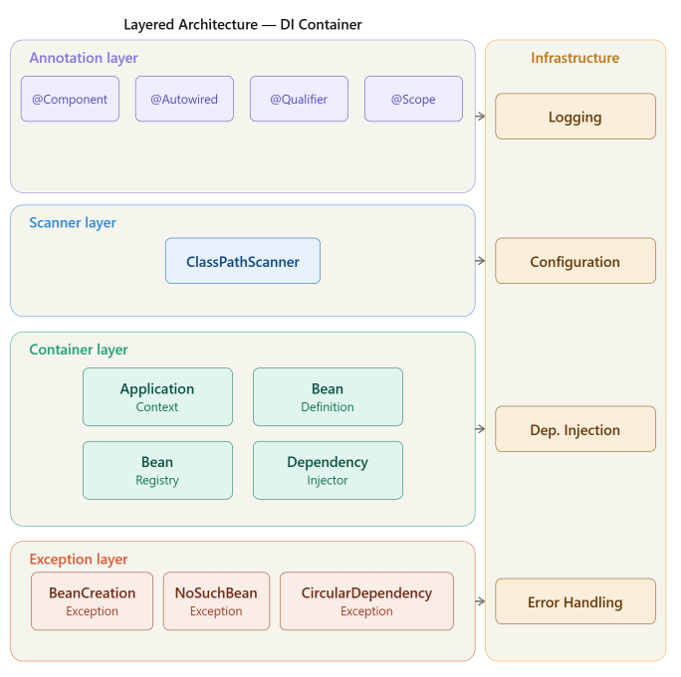
\includegraphics[width=0.7\linewidth]{images/architecture.png}
    \caption{Төслийн архитектур}
    \label{fig:architecture1}
\end{figure}
~\ref{fig:architecture1}-р зурагт annotation-д суурилсан
DI framework-ийн давхаргат архитектурыг харуулав.
Архитектур нь annotation давхарга, scanner давхарга,
container давхарга, exception давхарга гэсэн дөрвөн
үндсэн давхаргаас бүрдэх бөгөөд баруун талд infrastructure
хэсэг болох logging, configuration, dependency injection,
error handling үйлчилгээнүүд байрлана. Annotation давхарга
нь \texttt{@Component}, \texttt{@Autowired},
\texttt{@Qualifier}, \texttt{@Scope} annotation-уудыг
агуулж, scanner давхарга нь \texttt{ClassPathScanner}
ашиглан классуудыг илрүүлнэ. Container давхарга нь
\texttt{ApplicationContext}, \texttt{BeanDefinition},
\texttt{BeanRegistry}, \texttt{DependencyInjector} гэсэн
дөрвөн үндсэн бүрэлдэхүүнээс тогтох бол exception
давхарга нь \texttt{BeanCreationException},
\texttt{NoSuchBeanException},
\texttt{CircularDependencyException} гэсэн гурван
exception классаас бүрдэнэ.

\clearpage
\section{Activity Diagram}

Activity diagram нь системийн startup болон runtime үеийн ажиллагааны дарааллыг илэрхийлнэ. Эхлээд хэрэглэгч \texttt{ApplicationContext} үүсгэж, ClassPathScanner ашиглан package scanning хийнэ. Үүний дараа илэрсэн class бүрийг шалган \texttt{@Component} annotation бүхий class-уудаас \texttt{BeanDefinition} үүсгэн \texttt{BeanRegistry}-д бүртгэнэ.

Дараагийн шатанд singleton bean instance-үүдийг үүсгэж, \texttt{DependencyInjector} ашиглан dependency injection гүйцэтгэнэ. Хэрэв object үүсгэх явцад алдаа гарвал \texttt{BeanCreationException}, харин dependency шийдвэрлэх үед тойрог хамаарал илэрвэл \texttt{CircularDependencyException} шидэгдэнэ. Эдгээр тохиолдолд процесс шууд зогсоно.

Initialization амжилттай дууссаны дараа container бэлэн болж, хэрэглэгч \texttt{getBean()} аргаар шаардлагатай bean-ийг авах боломжтой болно. Хэрэв хүссэн bean олдохгүй бол \texttt{NoSuchBeanException} шидэгдэнэ.

\begin{figure}[H]
    \centering
    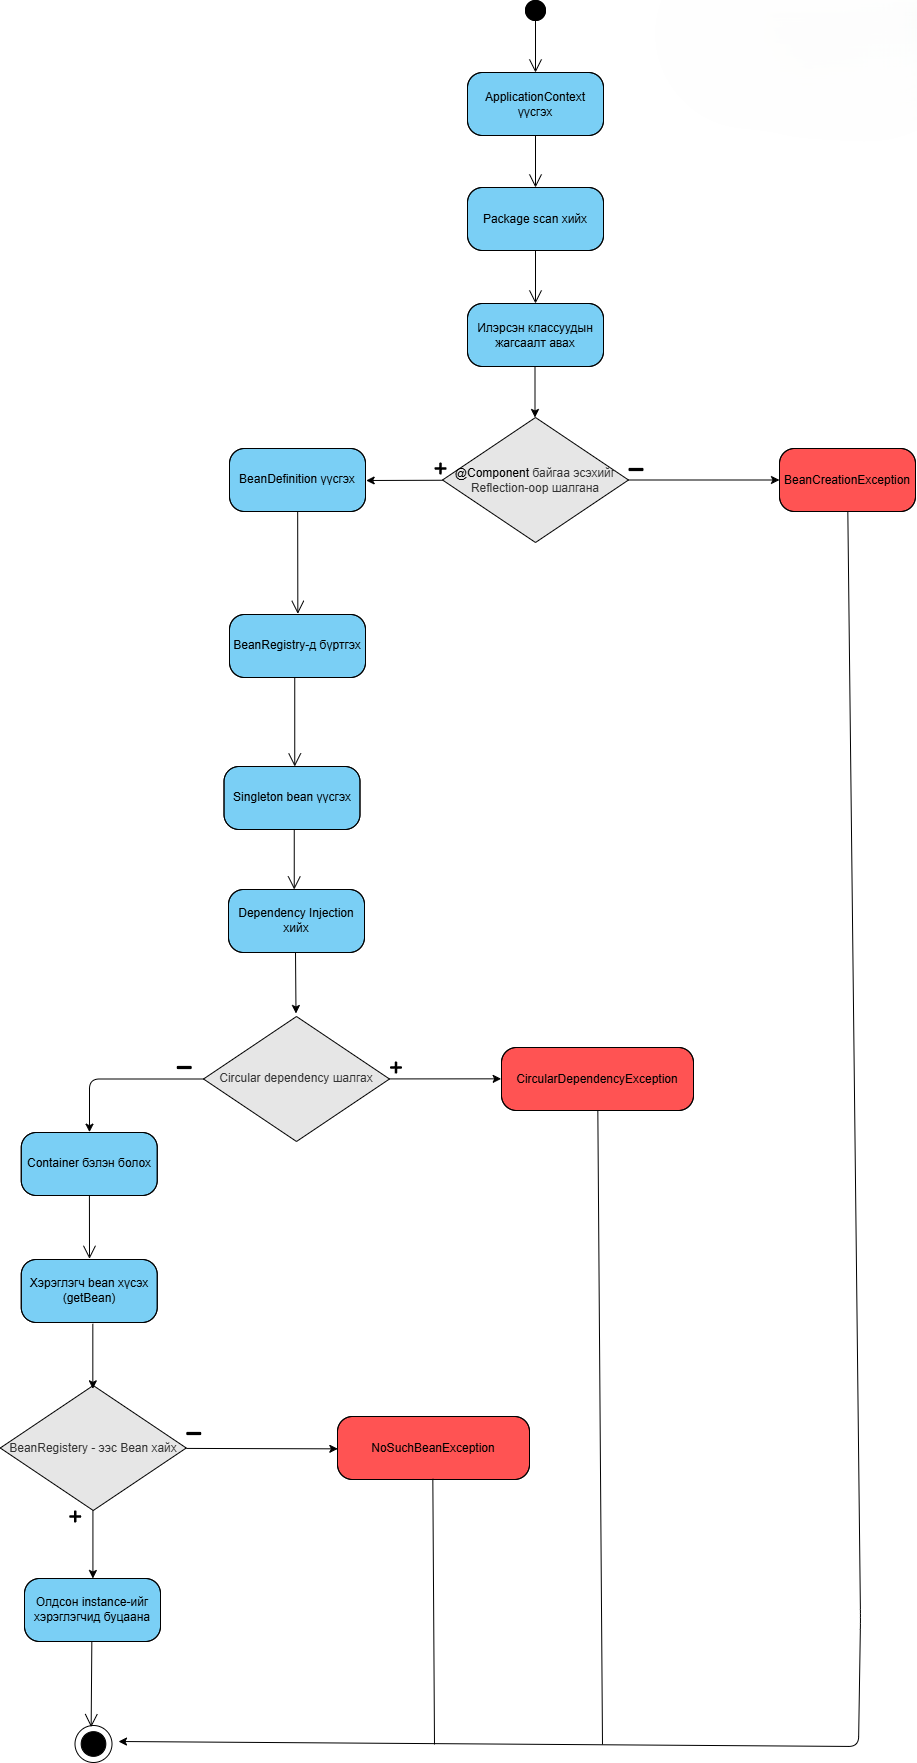
\includegraphics[width=0.5\linewidth]{images/Activity Diagram.png}
    \caption{Activity diagramm}
    \label{fig:activity-diagram}
\end{figure}
~\ref{fig:activity-diagram}-р зурагт DI framework-ийн
ажиллах дарааллын диаграммыг харуулав. Диаграмм нь
\texttt{ApplicationContext} үүсгэхээс эхлэн хэрэглэгчид
bean буцаах хүртэлх бүх үе шатыг дүрсэлнэ.

Эхний үе шатанд \texttt{ApplicationContext} үүсгэгдэж,
package scan хийгдэн илэрсэн классуудын жагсаалт авагдана.
Дараа нь \texttt{@Component} annotation байгааг Reflection
API ашиглан шалгах бөгөөд annotation олдохгүй тохиолдолд
\texttt{BeanCreationException} шидэгдэж процесс
зогсоно. Annotation олдсон тохиолдолд \texttt{BeanDefinition}
үүсгэгдэж \texttt{BeanRegistry}-д бүртгэгдэнэ.

Бүртгэлтийн дараа singleton bean-ууд урьдчилан үүсгэгдэж
dependency injection хийгдэнэ. Энэ үе шатанд circular
dependency шалгалт явагдах бөгөөд тойрог хамаарал илэрсэн
тохиолдолд \texttt{CircularDependencyException} шидэгдэнэ.
Тойрог хамаарал байхгүй бол container бэлэн болж
хэрэглэгч \texttt{getBean()} дуудах боломжтой болно.
\texttt{getBean()} дуудагдахад \texttt{BeanRegistry}-ээс
bean хайгдах бөгөөд bean олдохгүй тохиолдолд
\texttt{NoSuchBeanException} шидэгдэнэ. Bean олдвол
тухайн instance хэрэглэгчид буцаагдаж процесс амжилттай
дуусна.

\clearpage
\section{Sequence Diagram}

Sequence diagram нь объектуудын хоорондын харилцан ажиллагааны дарааллыг илэрхийлнэ. Эхлээд хэрэглэгч \texttt{ApplicationContext}-ийг үүсгэж, package scanning эхлүүлнэ. \texttt{ClassPathScanner} нь боломжит class-уудыг илрүүлж буцаана.

Үүний дараа \texttt{ApplicationContext} нь \texttt{@Component} annotation бүхий class-уудаас \texttt{BeanDefinition} үүсгэн \texttt{BeanRegistry}-д бүртгэнэ. Дараа нь singleton bean-үүдийг үүсгэж, \texttt{DependencyInjector} ашиглан dependency injection гүйцэтгэнэ.

Dependency injection хийх явцад шаардлагатай dependency-г \texttt{BeanRegistry}-ээс хайж олно. Хэрэв dependency шийдвэрлэх үед тойрог хамаарал илэрвэл \texttt{CircularDependencyException}, харин bean үүсгэх явцад алдаа гарвал \texttt{BeanCreationException} үүснэ.

Initialization дууссаны дараа хэрэглэгч \texttt{getBean()} дуудахад \texttt{ApplicationContext} нь \texttt{BeanRegistry}-ээс шаардлагатай bean-ийг хайж олно. Хэрэв bean олдвол instance-ийг буцааж, эсрэг тохиолдолд \texttt{NoSuchBeanException} шидэгдэнэ.

\begin{figure}[H]
    \centering
    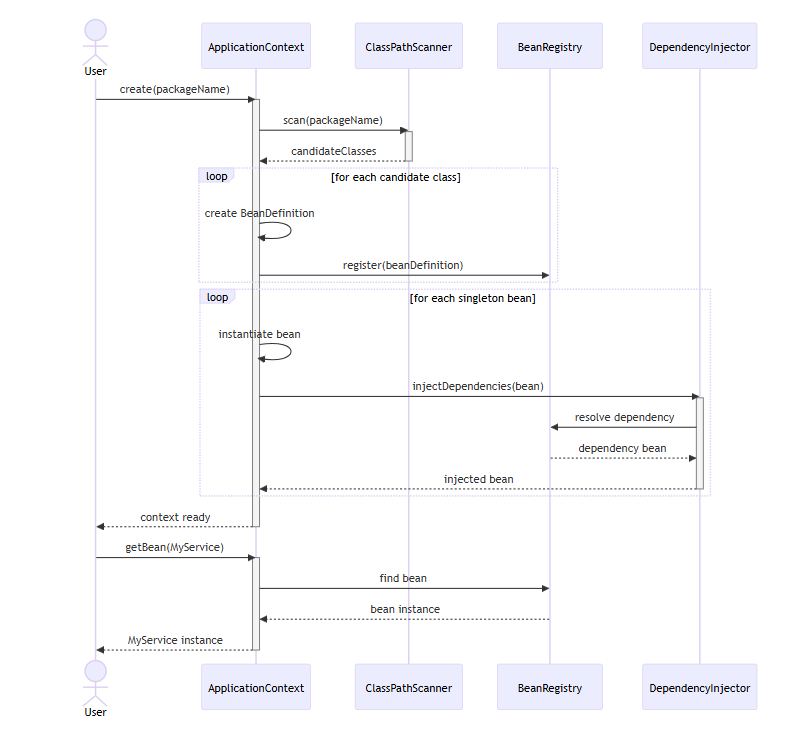
\includegraphics[width=0.5\linewidth]{images/sequence.png}
    \caption{Sequence diagramm}
    \label{fig:sequence-diagram}
\end{figure}
~\ref{fig:sequence-diagram}-р зурагт DI framework-ийн
startup болон bean авах үйл явцын дарааллын диаграммыг
харуулав. Диаграммд \texttt{User}, \texttt{ApplicationContext},
\texttt{ClassPathScanner}, \texttt{BeanRegistry},
\texttt{DependencyInjector} гэсэн таван оролцогч
харилцан үйлчилнэ.

Эхний үе шатанд хэрэглэгч \texttt{create(packageName)}
дуудахад \texttt{ApplicationContext} нь
\texttt{ClassPathScanner}-ийг ажиллуулж
\texttt{scan(packageName)} гүйцэтгэнэ. Scanner нь
\texttt{candidateClasses} буцааж өгөх бөгөөд
\texttt{ApplicationContext} нь candidate класс бүрийг
давтан \texttt{BeanDefinition} үүсгэж
\texttt{register(beanDefinition)} ашиглан
\texttt{BeanRegistry}-д бүртгэнэ.

Хоёрдугаар үе шатанд singleton bean бүрийг давтан
\texttt{instantiate bean} хийж, \texttt{injectDependencies(bean)}
ашиглан \texttt{DependencyInjector}-т дамжуулна.
\texttt{DependencyInjector} нь \texttt{BeanRegistry}-ээс
\texttt{resolve dependency} дуудаж шаардлагатай
\texttt{dependency bean}-г авч inject хийсний дараа
\texttt{injected bean}-г \texttt{ApplicationContext}-д
буцаана. Бүх singleton bean inject хийгдэж дууссаны
дараа \texttt{context ready} мэдэгдэл хэрэглэгчид
очиж container ашиглахад бэлэн болно.

Гуравдугаар үе шатанд хэрэглэгч
\texttt{getBean(MyService)} дуудахад
\texttt{ApplicationContext} нь \texttt{BeanRegistry}-ээс
\texttt{find bean} хайлт хийж олдсон
\texttt{bean instance}-г хэрэглэгчид
\texttt{MyService instance} хэлбэрээр буцаана.

\newpage

\section{A1 сайжруулалтын ажлын архитектурын уялдаа}

Нэмэлт хэрэгжүүлэлтийн A1 ажил нь энэхүү бүлэгт тодорхойлсон давхаргат архитектурыг өөрчлөх бус, харин түүний зөв зааглалыг баталгаажуулахад чиглэсэн. Өөрөөр хэлбэл annotation, scanner, container, exception гэсэн давхаргуудын хариуцлагыг хэвээр хадгалж, тухайн давхарга бүр ямар нөхцөлд ямар зан авир үзүүлэх ёстойг тестээр нотолсон нь энэ бүлгийн зохиомжийн шийдлийг практик түвшинд хамгаалсан гэж үзэж болно.

Ялангуяа \texttt{ApplicationContext} эхлэх үеийн \textit{scan $\rightarrow$ register $\rightarrow$ singleton preload $\rightarrow$ inject} урсгал нь activity болон sequence diagram-д тодорхойлсон логиктой бүрэн нийцэж байна. A1 ажлын хүрээнд энэ урсгалыг бүхэлд нь интеграцийн тестээр, харин доторх салбарласан нөхцлүүдийг нэгж тестээр тус тус баталгаажуулсан. Ингэснээр тухайн диаграммууд нь зөвхөн тайлбарын зураг биш, харин бодит хэрэгжүүлэлтийн дарааллыг илэрхийлж байгаа нь нотлогдож байна.


\renewcommand{\arraystretch}{1.25}
\scriptsize
\setlength{\tabcolsep}{3pt}
\begin{table}[H]
\centering
\caption{A1 ажлын архитектурын давхаргатай уялдсан байдал}
\label{tab:a1-architecture-alignment-fixed}
\begin{tabularx}{\textwidth}{|L{0.15\textwidth}|Y|Y|}
\hline
\textbf{Давхарга} & \textbf{A1 ажлын баталгаажуулсан зүйл} & \textbf{Архитектурын үр нөлөө} \\ \hline

Annotation &
\codeword{@Component}, \codeword{@Qualifier}, \codeword{@Scope}, \codeword{@Autowired}-ийн runtime хэрэглээг scanner болон injector-ийн тестээр баталсан &
Annotation давхарга нь зөвхөн мета мэдээлэл дамжуулах үүргээ цэвэр хадгалж байна. \\ \hline

Scanner &
Package байхгүй, interface, component биш класс, custom/default bean нэр, scope уншилт зэрэг урсгалыг тусад нь шалгасан &
Scanner давхаргын шүүлт, илрүүлэлтийн логик бие даасан модуль гэдэг нь баталгаажсан. \\ \hline

Container &
Bean бүртгэл, singleton cache, төрлөөр хайлт, circular dependency илрүүлэлт, fail-fast lookup-ийг баталсан &
Container давхарга системийн төв удирдлага хэвээр байж, бусад давхаргын үр дүнг нэгтгэн зохицуулж байна. \\ \hline

Exception &
Алдааны мэдэгдэлд bean нэр, төрөл, шалтгаан, боломжит candidate-уудыг тусгасан &
Fail-fast архитектур зөвхөн exception шидэх биш, харин оношлоход ашигтай мэдээлэл өгөх түвшинд хэрэгжсэн. \\ \hline

Интеграцийн урсгал &
Dependency injection, qualifier, scope, bean lookup, bean creation failure, circular dependency-г end-to-end түвшинд шалгасан &
Activity diagram болон sequence diagram-д дүрсэлсэн урсгал бодит систем дээр тогтвортой хэрэгжиж байгааг харуулсан. \\ \hline

\end{tabularx}
\end{table}
\normalsize
\renewcommand{\arraystretch}{1}


Иймээс A1 сайжруулалтын ажлыг архитектурын үүднээс авч үзвэл энэ нь шинэ бүтэц нэмсэн ажил бус, харин 3-р бүлгээр сонгосон layered architecture-ийн зөв шийдэл, тестлэгдэх чадвар, fail-fast шинж чанарыг баталгаажуулсан чанарын бэхжилтийн шат юм.

\section{A3 dependency tree ажлын архитектурын уялдаа}

Нэмэлт хэрэгжүүлэлтийн A3 ажил нь layered architecture-ийг өөрчлөх бус, харин \texttt{container} давхаргын дотор dependency graph боловсруулах шинэ дэд модуль нэмсэн архитектурын өргөтгөл юм. Энэ өргөтгөлийн хүрээнд \texttt{DependencyNode}, \texttt{DependencyTreeBuilder}, \texttt{DependencyTreeExporter}, \texttt{DependencyTreeHtmlExporter} гэсэн дөрвөн шинэ бүрэлдэхүүн нь bean registry, annotation inspection, dependency resolution-ийн одоо байгаа үр дүнд тулгуурлан graph representation боловсруулдаг болсон. Иймээс A3 нь шинэ бие даасан давхарга биш, харин container давхаргын ``өөрийгөө тайлбарлах'' болон ``оношлох'' боломжийг нэмсэн дотоод дэд систем гэж үзэж болно.

Энэ дэд системийн урсгал дараах байдлаар ажиллана. \texttt{ApplicationContext} startup үед scanner-аар классуудыг илрүүлж, registry-д bean-үүдийг бүртгэж, singleton bean-үүдийг үүсгэсний дараа dependency tree builder-ийг ажиллуулна. Tree builder нь registry-д буй \texttt{BeanDefinition}-уудыг уншиж node-ууд үүсгэн, \texttt{@Autowired} field бүрээр dependency холбоос тогтооно. Үүний дараа DFS алгоритмаар cycle илрүүлэх, console tree хэвлэх, JSON export гаргах, HTML dashboard үүсгэх зэрэг exporter ба visualization pipeline ажиллах боломжтой болно. Энэ нь activity болон sequence diagram-д байсан startup урсгал дээр ``scan $\rightarrow$ register $\rightarrow$ preload $\rightarrow$ inject'' дарааллаас хойш ``build tree $\rightarrow$ export/visualize'' гэсэн шинэ шат нэмэгдсэнийг илэрхийлж байна.

\begin{table}[H]
\centering
\small
\setlength{\tabcolsep}{4pt}
\caption{A3 ажлын архитектурын давхаргатай уялдсан байдал}
\label{tab:a3-architecture-alignment}
\renewcommand{\arraystretch}{1.3}
\begin{tabularx}{\textwidth}{|L{0.16\textwidth}|L{0.26\textwidth}|Y|}
\hline
\textbf{Давхарга / бүрэлдэхүүн} & \textbf{A3 хүрээнд нэмэгдсэн зүйл} & \textbf{Архитектурын үр нөлөө} \\ \hline
Container layer & \texttt{DependencyNode}, \texttt{DependencyTreeBuilder}, \texttt{DependencyTreeExporter}, \texttt{DependencyTreeHtmlExporter} & Container нь зөвхөн bean удирдах биш, мөн dependency graph боловсруулах, экспортлох, runtime дүрслэх шинэ чадвартай болсон. \\ \hline
ApplicationContext & Tree lifecycle integration & Startup төгсгөлд tree үүсгэж, \texttt{getTreeBuilder()}-ээр хэрэглээнд нээлттэй болгосноор container-ийн төлөвийг ажиглах боломж бүрдсэн. \\ \hline
Annotation layer & \texttt{@EnableIoC(visualize = true)} & Visualization-г main startup declaration түвшинд идэвхжүүлэх hook нэмэгдэж, Spring Boot-той төстэй declarative startup хэв маяг үүссэн. \\ \hline
Scanner layer & Registry-д өгөгдөл бэлтгэх & Scanner-ийн илрүүлсэн bean-үүд graph-ын node болох тул scanner давхаргын үр дүн архитектурын хувьд илүү үнэ цэнтэй болж хувирсан. \\ \hline
Exception / fail-fast behavior & DFS cycle reporting & Circular dependency-г startup ба tree analysis түвшинд хоёуланд нь илрүүлэх замаар fail-fast шинж чанарыг архитектурын түвшинд бэхжүүлсэн. \\ \hline
Testing architecture & Integration + unit validation & Dependency graph ба startup visualization-ийг тусгаарлан турших боломжтой болж, layered architecture-ийн testability нэмэгдсэн. \\ \hline
\end{tabularx}
\end{table}

Хүснэгт~\ref{tab:a3-architecture-alignment}-оос харахад A3 ажил нь annotation, scanner, container, exception гэсэн өмнөх давхаргуудын зааглалыг эвдээгүй, харин container давхаргын дотор dependency structure боловсруулах хариуцлагыг шинээр тодорхойлсон байна. Ингэснээр системийн үндсэн startup урсгал архитектурын хувьд өөрчлөгдөөгүй ч, түүний үр дүнг хүний ойлгохуйц хэлбэрээр шинжлэх шинэ архитектурын capability нэмэгдсэн гэж үзэж болно.

Энэхүү зохиомжийн өөрчлөлтийн үр дүнд дараах баримт бичгийн шинэчлэлтүүд шаардлагатай болсон.
\begin{itemize}
    \item Layered architecture diagram-д container layer дотор dependency tree submodule-ийг нэмэх;
    \item Activity diagram-д startup төгсгөлд \textit{Build dependency tree} болон \textit{Export / Visualize} алхам нэмэх;
    \item Sequence diagram-д \texttt{ApplicationContext} -- \texttt{DependencyTreeBuilder} -- exporter урсгалыг тусгах;
    \item Багцын зохион байгуулалтын хүснэгтэд dependency visualization pipeline-ийн тайлбарыг нэмэх;
    \item CRC картын түвшинд \texttt{ApplicationContext}-ийн шинэ responsibility болгон dependency tree lifecycle удирдлагыг оруулах.
\end{itemize}

\section{Бүлгийн дүгнэлт}

Энэ бүлэгт annotation-д суурилсан dependency injection framework-ийн архитектурын зохиомжийг боловсруулж, системийн давхаргат бүтэц болон түүний динамик ажиллагааг Activity болон Sequence диаграммуудаар илэрхийллээ. Энэхүү архитектур нь системийн ойлгомжтой байдал, өргөтгөх боломж, тестлэх чадварыг сайжруулсан оновчтой шийдэл болж байна. Мөн A1 сайжруулалтын ажлын хүрээнд уг зохиомжийг эвдэлгүйгээр давхарга тус бүрийн зан авирыг тестээр баталсан нь энэ бүлэгт тодорхойлсон архитектурын шийдлийн бодит хэрэгжилтийн нотолгоо боллоо.
